%% ACM sigconf draft for MARVIN
\documentclass[sigconf]{acmart}

%% TODO: replace with actual conference information
\setcopyright{acmlicensed}
\copyrightyear{2025}
\acmYear{2026}
\acmDOI{XXXXXXX.XXXXXXX}
\acmConference[TEI SDC '26]{TEI Student Design Challenge}{March, 2026}{Chicago, Illinois}
\acmISBN{978-1-4503-XXXX-X/2026/06}

\AtBeginDocument{\providecommand\BibTeX{{Bib\TeX}}}

%% Remove for camera ready if not needed
% \citestyle{acmauthoryear}

\begin{document}

\title{MARVIN: Remote Teleoperation of a Dual-Arm Upper-Body Avatar Robot}
\subtitle{Real-time human motion mirroring with client-side ML and ROS2}

%% Authors
\author{Jaeho Cho}
\authornote{Both authors contributed equally to this research.}
\email{jaeho.cho@cooper.edu}
\affiliation{%
  \institution{The Cooper Union for the Advancement of Science and Art}
  \city{New York}
  \state{New York}
  \country{USA}
}
\author{Sophia Klymchuk}
\authornotemark[1]
\email{sophia.klymchuk@cooper.edu}
\affiliation{%
  \institution{The Cooper Union for the Advancement of Science and Art}
  \city{New York}
  \state{New York}
  \country{USA}
}

\renewcommand{\shortauthors}{Last}

%% Abstract
\begin{abstract}
We present MARVIN, a dual-arm teleoperational robot that mirrors a human operator's upper-body motion in real time using just a standard webcam. Client-side MediaPipe models extract 3D pose and hand landmarks, which are transmitted via websocket to a ROS2-MoveIt servoing stack that commands two OpenManipulator-X arms. We detail perception-to-actuation mappings, including geometric formulations for shoulder flexion, shoulder abduction/adduction, and elbow flexion, and describe a web interface that enables intuitive interaction. We report latency, accuracy, and user study results from local and remote operation, discuss safety and failure modes, and outline pathways toward full-body telepresence.
\end{abstract}

%%
%% The code below is generated by the tool at http://dl.acm.org/ccs.cfm.
%%
\begin{CCSXML}
<ccs2012>
   <concept>
       <concept_id>10010583</concept_id>
       <concept_desc>Hardware</concept_desc>
       <concept_significance>500</concept_significance>
       </concept>
 </ccs2012>
\end{CCSXML}

\ccsdesc[500]{Hardware}

\keywords{teleoperation, human-robot interaction, ROS2, MoveIt, MediaPipe}

% TODO: replace with dates
\received{NA}
\received[revised]{NA}
\received[accepted]{NA}

\maketitle

\section{Introduction}
MARVIN is a teleoperational robot that mirrors the upper-body movements of a human operator in real time. Operation works via a local webcam or a remote connection. For remote operation, a web application captures the user's webcam stream for pose landmarking, enabling MARVIN to act as a physical avatar across any distance.

\section{SDC 2026 Theme: Sensory Rituals}
MARVIN explores the theme of Sensory Rituals through the design of a remotely operated robot that reintroduces physicality into digital communication. In contemporary society, much of interpersonal interaction occurs through screen-based interfaces, which often diminish embodied and sensory engagement. The proposed system seeks to restore a sense of presence and tactility within virtual meetings by allowing users to inhabit a physical robot equipped with two controllable robotic arms.

The act of remotely manipulating the robot becomes a new form of ritualized sensory engagement-- practice that bridges physical and digital domains to cultivate social connection, attentional focus, and emotional resonance. By translating human gestures into robotic motion, the system enables users to perform actions, express intention, and interact with shared physical environments. This transforms otherwise disembodied virtual communication into an embodied, tangible experience.

Furthermore, the robot’s accessibility--requiring only a standard webcam and web interface--extends this ritual of presence to anyone, anywhere, without technical barriers. This inclusivity positions the system as a tool for fostering shared sensory experience and collective grounding in hybrid or remote contexts. Through its integration of tangible interaction, telepresence, and accessible design, the project proposes that sensory rituals need not be confined to traditional or personal practices; they can also emerge from technological mediation that reconnects individuals to the physical world and to one another.

% \section{Related Work}
% TODO: 

\section{Hardware}
MARVIN uses components from the ROBOTIS OpenManipulator-X platform. Each arm has 5 DOF and is powered by Dynamixel XM430-W350 servos. We employ two arms attached to an aluminum-beam torso and powered via a Dynamixel U2D2 power hub.

\section{Software}
MARVIN runs on the Humble distribution of ROS2. High-level motion is handled by MoveIt, which translates user commands into low-level commands sent to Dynamixel controllers. A custom URDF/Xacro model encodes simultaneous kinematics, inertias, and control interfaces for both arms.

\subsection{Pose Detection}
OpenCV interfaces a MediaPipe-based pose detector to extract normalized 3D joint landmarks from a webcam stream \cite{noauthor_mediapipe_nodate}. We use shoulder (11,12), elbow (13,14), wrist (15,16), and hip (23,24) landmarks to compute joint angles that are then mapped to MARVIN's kinematic model.

\begin{figure}[htbp]
  \centering
  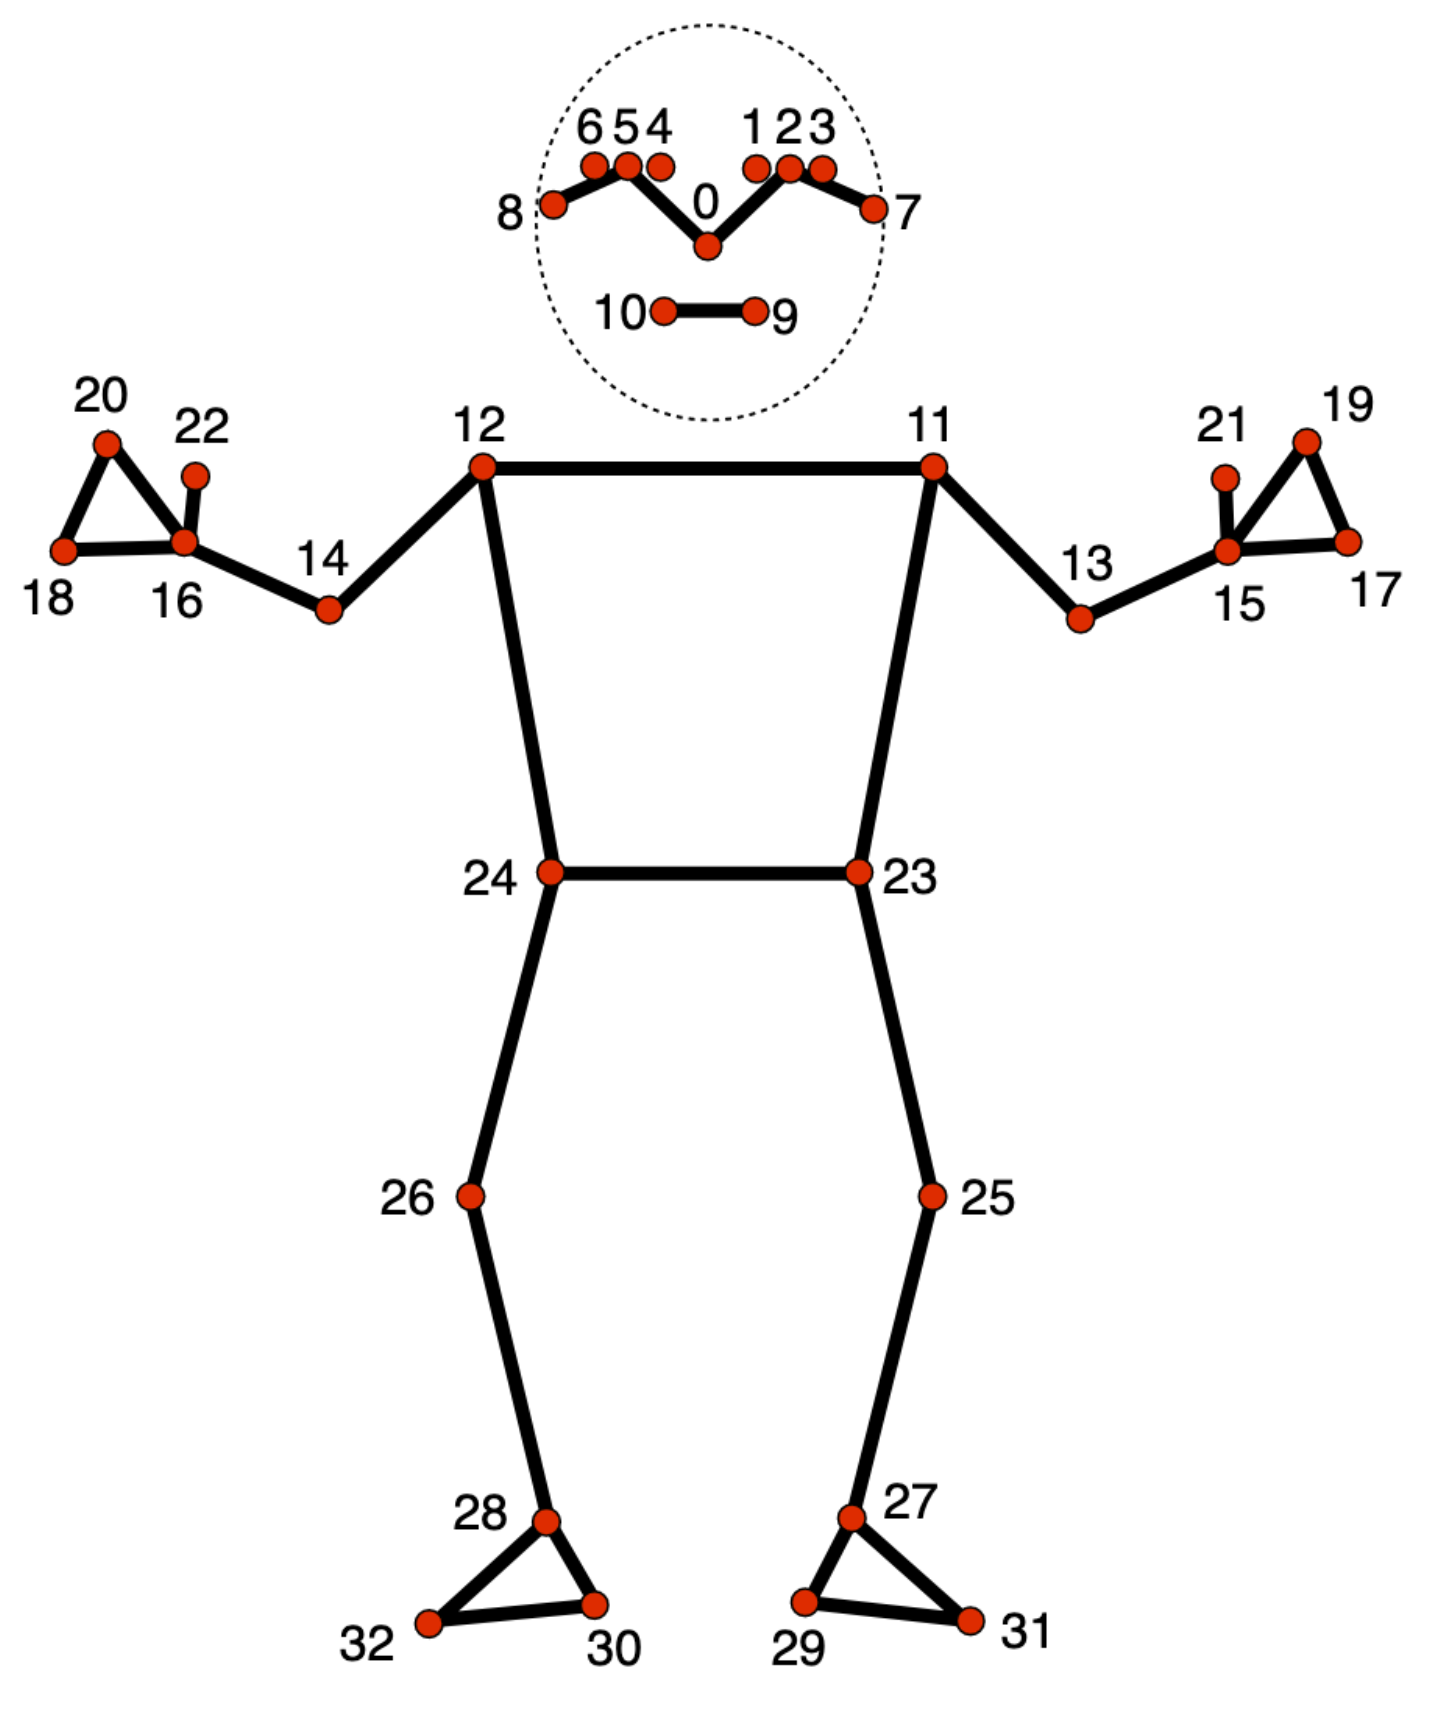
\includegraphics[width=\linewidth]{assets/pose-landmarks.png}
  \caption{MediaPipe Pose Landmarks. The pose landmarker model tracks 33 body landmark locations, representing the approximate location of the labeled body parts.}
  \Description{A diagram of a human figure with 33 labeled landmarks, including shoulders, elbows, wrists, hips, knees, and ankles.}
  \label{fig:pose-landmarks}
\end{figure}

\subsubsection{Shoulder Flexion}
Let $S$ (shoulder), $E$ (elbow), $H$ (same-side hip), $H_{opp}$ (opposite hip).
\begin{displaymath}
  \mathbf{u}=E-S,\quad \mathbf{v}=H-S,\quad \mathbf{h}=H_{opp}-H,\quad \hat{\mathbf{n}}=\frac{\mathbf{h}}{\lVert\mathbf{h}\rVert}
\end{displaymath}
Project onto the midline plane orthogonal to $\hat{\mathbf{n}}$:
\begin{displaymath}
\mathbf{u}_\pi=\mathbf{u}-(\mathbf{u}\cdot\hat{\mathbf{n}})\,\hat{\mathbf{n}},\quad
\mathbf{v}_\pi=\mathbf{v}-(\mathbf{v}\cdot\hat{\mathbf{n}})\,\hat{\mathbf{n}}.
\end{displaymath}
Flexion:
\begin{equation}
\alpha=\arccos \!\left( \frac{\mathbf{u}_\pi \cdot \mathbf{v}_\pi}{\lVert\mathbf{u}_\pi\rVert\, \lVert\mathbf{v}_\pi\rVert} \right)\,.
\end{equation}
Map $\alpha$ to shoulder flexion/extension joint ($J_1$).

\subsubsection{Shoulder Adduction/Abduction}
Let $\mathbf{u}=E-S$, $\hat{\mathbf{n}}$ as above. Project $\mathbf{u}$:
\begin{displaymath}
\mathbf{u}_\pi=\mathbf{u}-(\mathbf{u}\cdot\hat{\mathbf{n}})\,\hat{\mathbf{n}}.
\end{displaymath}
Adduction magnitude:
\begin{equation}
\beta=\arccos \!\left( \frac{\mathbf{u}\cdot\mathbf{u}_\pi}{\lVert\mathbf{u}\rVert\, \lVert\mathbf{u}_\pi\rVert} \right)\,.
\end{equation}
Signed ab/adduction can be obtained from $\operatorname{sign}\big((\mathbf{u}\times\mathbf{u}_\pi)\cdot\hat{\mathbf{n}}\big)$. Map to $J_2$.

\subsubsection{Elbow Flexion}
Let $\mathbf{u}=E-S$ and forearm $\mathbf{f}=E-W$. Then
\begin{equation}
\theta=\arccos \!\left( \frac{\mathbf{u}\cdot\mathbf{f}}{\lVert\mathbf{u}\rVert\, \lVert\mathbf{f}\rVert} \right)\,.
\end{equation}
Map $\theta$ to elbow joint $J_3$.

\subsubsection{Hand Open/Close}
Using the Hand Landmarker, define a reference length from wrist (0) to middle-finger MCP (9). Mark a hand as open if fewer than three fingertips among indices \{4,8,12,16,20\} lie closer to the wrist than the reference. Publish binary open/closed to drive the gripper.

\begin{figure}[htbp]
  \centering
  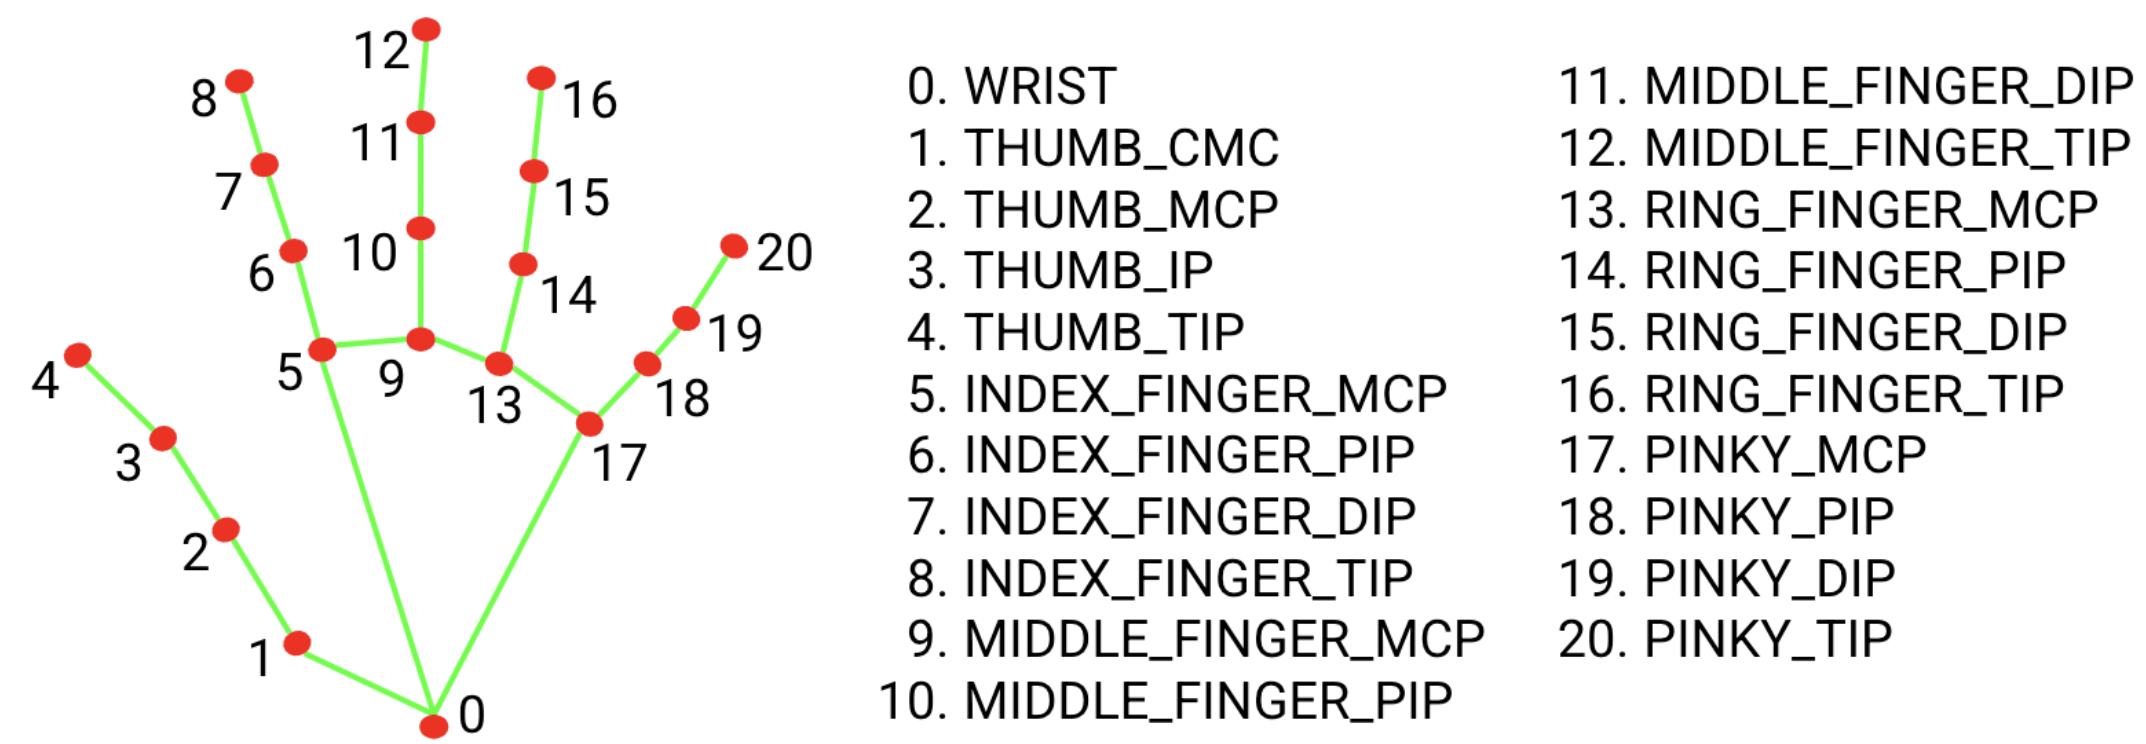
\includegraphics[width=\linewidth]{assets/hand-landmarks.png}
  \caption{MediaPipe Hand Landmarks. The hand landmark model bundle detects the keypoint localization of 21 hand-knuckle coordinates within the detected hand regions.}
  \Description{A diagram of a hand with 21 labeled landmarks, including wrist, palm, and finger joints.}
  \label{fig:hand-landmarks}
\end{figure}

\subsection{Control}
We use MoveIt real-time servoing with two independent kinematic chains, one per arm. Each chain is associated with a servoing node that subscribes to desired joint velocities. Desired velocities are computed from the error between detected target joint angles and current joint states from the \texttt{/joint\_states} topic. Errors are scaled by gains and sent as \texttt{JointJog} commands.

\section{Website}
The MediaPipe Pose \& Hands — ROSBridge webpage functions as the browser-based front end of MARVIN’s remote teleoperation system. It captures the user’s webcam stream, performs on-device pose and hand landmark inference, and transmits the resulting kinematic data to the ROS2 backend in real time. The interface also embeds a live video stream of the robot, allowing visual feedback during operation. Implemented entirely in client-side JavaScript using the MediaPipe Tasks API, the system requires no native installation or external dependencies. A compact control panel enables users to start or stop the camera, select inference model complexity, and toggle streaming to the ROSBridge server, which exposes \texttt{pose\_landmarks} and \texttt{hand\_landmarks} topics for downstream motion control.

Detected landmarks are overlaid directly on the live video feed, and the interface reports both frame rate and end-to-end latency to the ROSBridge server, enabling quantifiable performance evaluation under varying network conditions. Hand openness is computed geometrically from landmark distances, and both hand-state and pose data are serialized into ROS-compatible JSON messages. This design supports seamless integration with MARVIN’s MoveIt servoing pipeline, where landmark-derived joint angles are mapped to actuator commands for real-time mirroring of human motion.

\begin{figure}[htbp]
  \centering
  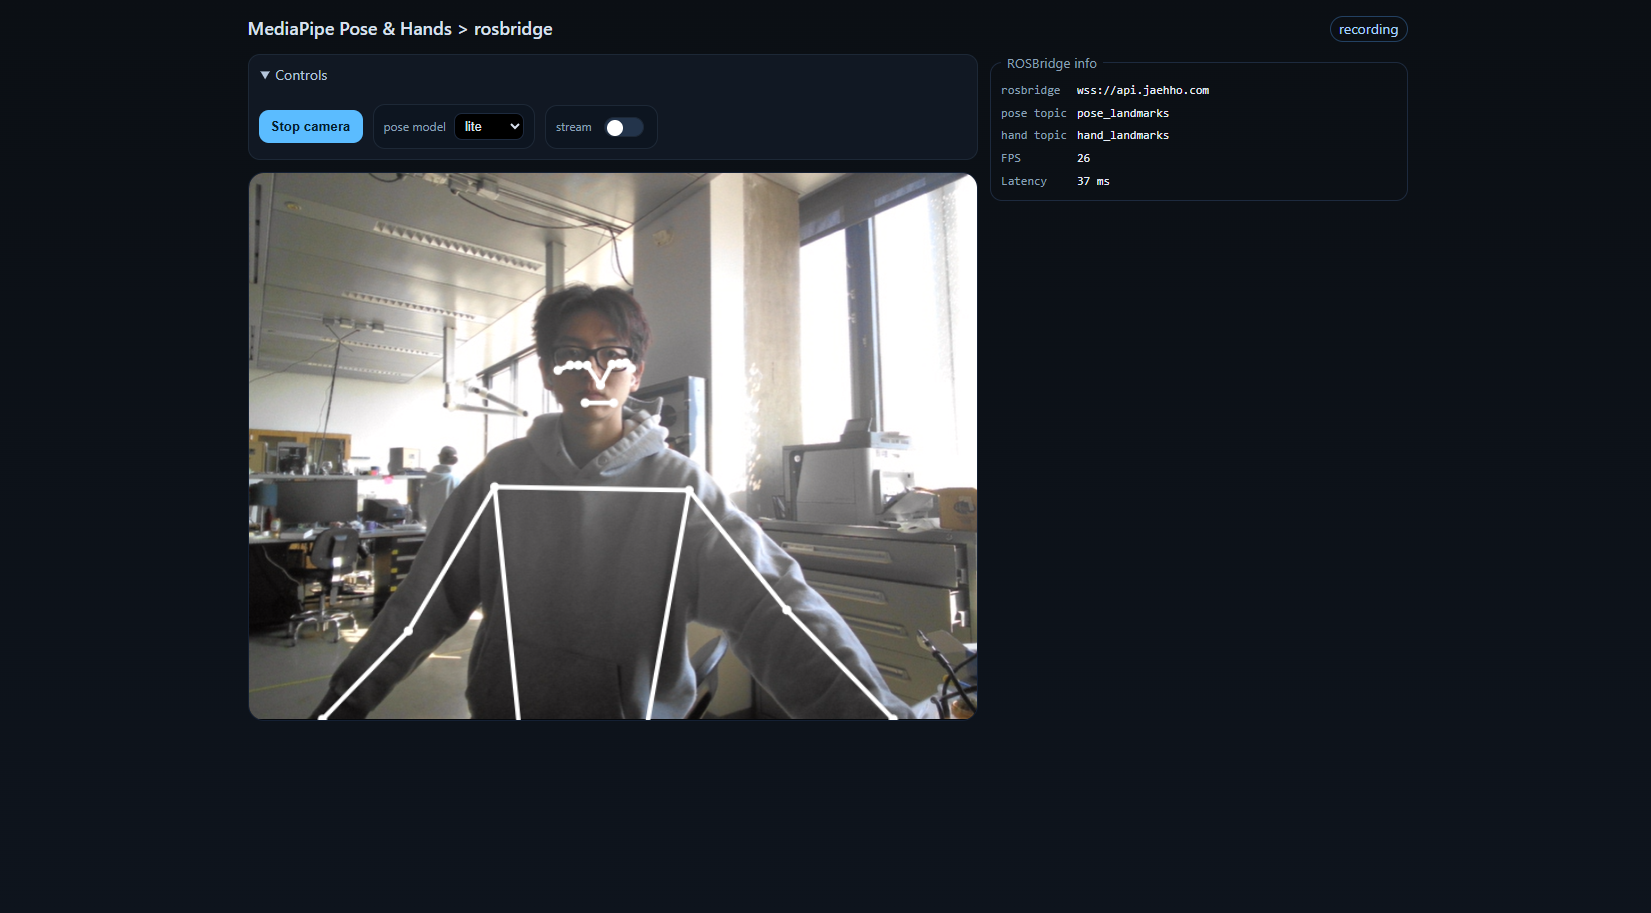
\includegraphics[width=\linewidth]{assets/web-ui}
  \caption{Browser UI for teleoperation. TODO: elaborate.}
  \Description{A screenshot of the web interface showing video feed, control buttons, and status indicators.}
  \label{fig:ui}
\end{figure}

\begin{figure}[htbp]
  \centering
  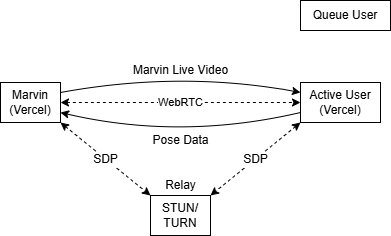
\includegraphics[width=\linewidth]{assets/system-diagram}
  \caption{ROS rqt graph overview. TODO: elaborate.}
  \Description{TODO}
  \label{fig:system}
\end{figure}

\begin{figure}[htbp]
  \centering
  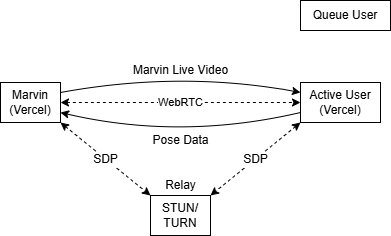
\includegraphics[width=\linewidth]{assets/system-diagram.png}
  \caption{Communication pipeline and timing. TODO: elaborate.}
  \Description{TODO}
  \label{fig:pipeline}
\end{figure}

\begin{figure}[htbp]
  \centering
  \includegraphics[width=\linewidth]{assets/marvin}
  \caption{MARVIN hardware. Front and oblique views of the dual-arm upper-body platform with aluminum-beam torso, two 5-DOF OpenManipulator-X arms, and parallel grippers. Insets show Dynamixel XM430-W350 servos, U2D2 hub, and mounting.}
  \Description{Photographs of MARVIN from multiple angles highlighting mechanical structure, actuators, and end-effectors.}
  \label{fig:photos}
\end{figure}

% \section{Operation and User Study}
% We tested MARVIN in local and remote operation with volunteers. We describe protocol, tasks, and measurements.

% \subsection{Protocol}
% % Fill with your actual study design
% Participants performed pick-and-place and reach-to-touch tasks. Conditions: (i) local network, (ii) remote over the public internet. Metrics: task success, completion time, path length, perceived workload (NASA-TLX), presence, and perceived responsiveness.

\subsection{Latency}\label{sec:latency}
We define end-to-end latency as camera exposure to actuator motion onset. We report median and 95th percentile latencies for both conditions, along with landmark inference time and ROSBridge transmission time.

\begin{table}[htbp]
  \caption{Performance summary (illustrative; replace with measured data).}
  \label{tab:perf}
  \begin{tabular}{lrr}
    \toprule
    Metric & Local & Remote \\
    \midrule
    End-to-end latency (ms) &  \textit{TODO} & \textit{TODO} \\
    Pose inference (ms/frame) & \textit{TODO} & \textit{TODO} \\
    FPS (avg) & \textit{TODO} & \textit{TODO} \\
    Task success rate (\%) & \textit{TODO} & \textit{TODO} \\
    NASA-TLX (0--100) & \textit{TODO} & \textit{TODO} \\
    \bottomrule
  \end{tabular}
\end{table}

\section{Safety and Limits}
We enforce velocity, position, and torque limits at the controller. We apply workspace clamping and filtering of pose outliers using temporal smoothing. Failure modes include landmark jitter, partial occlusion, and network loss. A dead-man switch disables actuation when no fresh landmarks arrive within a timeout.

% \section{Results}
% % Summarize quantitative and qualitative findings after you add data
% We observe that local operation achieves lower latency and higher success rates than remote. Participants report higher presence locally. Grasp success correlates with hand-state classification accuracy.

\section{Discussion}
MARVIN demonstrates that fully client-side inference is viable for dual-arm mirroring. Remaining gaps include wrist pronation supination estimation, depth ambiguity in monocular input, and gripper force control. Future work includes fusing depth, adding self-calibration, and extending to mobile bases for whole-body telepresence.

\section{Ethical and Societal Impact}
Telepresence expands access but raises safety and privacy concerns. We log minimal data, anonymize telemetry where possible, and provide hard e-stop. Future deployments must consider operator authentication and bystander consent in public spaces.

\section{Conclusion}
We provided a browser-first teleoperation system that minimizes setup while retaining precise, low-latency control of a dual-arm avatar robot. We plan to release code and evaluation datasets.

\begin{acks}
We thank the Cooper Union community for volunteering and supporting facilities.
\end{acks}

\bibliographystyle{ACM-Reference-Format}
\bibliography{references}

\appendix
\section{Angle Mapping and Calibration}
We recommend a short calibration where the operator performs canonical poses to establish shoulder plane and joint-neutral offsets. Offsets are subtracted from observed angles before mapping to robot joints.

\section{Implementation Details}
Browser stack: TypeScript, WebAssembly MediaPipe Tasks. ROSBridge schema and message formats are in the repository. Build and launch instructions for both simulation (Gazebo/Ignition) and hardware are provided.

\end{document}
